\question*{
    \begin{center}
        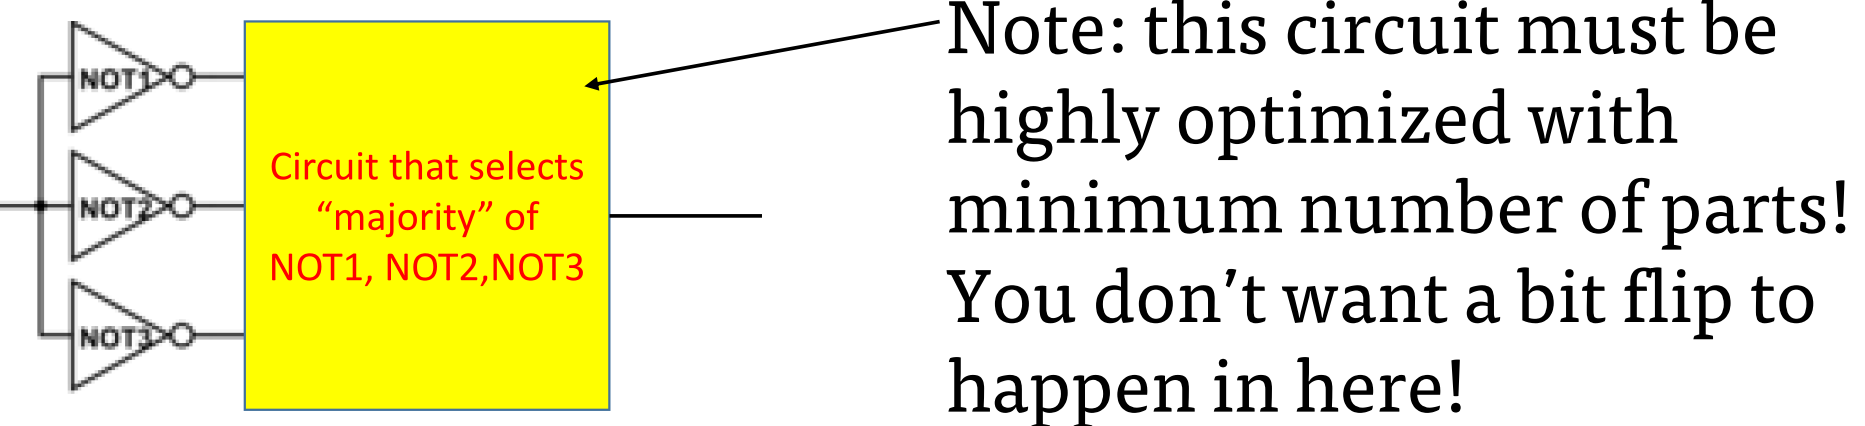
\includegraphics[width=0.5\textwidth]{fig/design_diagram.png}
    \end{center}
Design a minimal circuit that goes into the 
yellow box above. It must take 3 digital inputs, 
and produce 1 digital output. Output = value that matches at least 
two of the inputs. i.e. Output is the 'majority value' of the 3 inputs. 
Even if one of the inputs is wrong due to SEU, 
we will still get the correct answer. \hfill \textbf{[30]}}

We can construct a simple minimal logic circuit using a Karnaugh
Map. First, we establosh the form of the circuit and construct a
target truth table.

\begin{figure}[ht]
    \centering
    \begin{tikzpicture}
    
\end{tikzpicture}
    \caption{Expected Circuit}
    \label{fig:black-box-circ}
\end{figure}

And, the truth table for $f(A, B, C)$

\begin{figure}[ht]
    \centering
    \begin{tabular}{c c c | c}
        %headings
        $A$   &   $B$   &   $C$   &   $f(A, B, C)$ \\ \hline
        0     &    0    &    0    &         0      \\
        0     &    0    &    1    &         0      \\
        0     &    1    &    0    &         0      \\
        0     &    1    &    1    &         1      \\
        1     &    0    &    0    &         0      \\
        1     &    0    &    1    &         1      \\
        1     &    1    &    0    &         1      \\
        1     &    1    &    1    &         1      %
        
    \end{tabular}
    \label{fig:truth-table}
\end{figure}

Minimizing $f$ using a Karnaugh Map

\begin{figure}[h]
    \centering

    \begin{karnaugh-map}[4][2][1][$AB$][$C$]
        \manualterms{0,0,0,1,0,1,1,1}
        \implicant{3}{7}
        \implicant{5}{7}
        \implicant{7}{6}
    \end{karnaugh-map}
    
    \label{fig:kmap}
\end{figure}

we get $f(A, B, C) = AB + BC + CA$.
